% GGS 662 Assignment 3 -- research proposal deck (5-minute talk).
% Build (from this folder), run twice:
%   pdflatex -interaction=nonstopmode -output-directory=.build assignment3_proposal.tex && cp .build/assignment3_proposal.pdf .
% Content sources: ../lab_inputs.ipynb (A3, L1, H1-H6) and ../outputs/*.md (agent stages).
% Red TODOs must be resolved before submitting.
\documentclass[aspectratio=169,11pt]{beamer}
\usetheme[progressbar=frametitle,numbering=fraction,block=fill,sectionpage=none]{metropolis}
\usepackage[T1]{fontenc}
\usepackage[sfdefault,scale=0.93]{FiraSans}
\usepackage[scale=0.88]{FiraMono}
\usepackage{booktabs}
\usepackage{colortbl}
\usepackage{tabularx}
\usepackage{array}
\usepackage{tikz}
\usetikzlibrary{positioning,arrows.meta}

% ---- palette (same as the Assignment 2 deck)
\definecolor{navy}{HTML}{102A43}
\definecolor{ink}{HTML}{1F2933}
\definecolor{muted}{HTML}{616E7C}
\definecolor{amber}{HTML}{C2410C}
\definecolor{teal}{HTML}{0F766E}
\definecolor{failred}{HTML}{B91C1C}
\definecolor{paper}{HTML}{FBFAF7}
\definecolor{rule}{HTML}{E4E0D8}
\definecolor{tealtint}{HTML}{E6F2F1}
\definecolor{ambertint}{HTML}{FDF0E7}

\setbeamercolor{normal text}{fg=ink,bg=paper}
\setbeamercolor{background canvas}{bg=paper}
\setbeamercolor{frametitle}{bg=paper,fg=navy}
\setbeamercolor{progress bar}{fg=teal,bg=rule}
\setbeamercolor{title separator}{fg=teal}
\setbeamercolor{alerted text}{fg=amber}
\setbeamercolor{block title}{bg=tealtint,fg=navy}
\setbeamercolor{block body}{bg=white,fg=ink}
\setbeamercolor{page number in head/foot}{fg=muted}
\setbeamercolor{footline}{fg=muted}
\setbeamercolor{palette primary}{bg=navy,fg=paper}
\setbeamerfont{frametitle}{size=\large,series=\bfseries}
\setbeamerfont{block title}{series=\bfseries}
\setbeamerfont{footline}{size=\tiny}
\setbeamerfont{page number in head/foot}{size=\tiny}
\setbeamertemplate{frame footer}{GGS 662 \enskip·\enskip Assignment 3 \enskip·\enskip What does an agent add?}
\setbeamertemplate{itemize item}{\textcolor{teal}{\small$\blacktriangleright$}}
\setbeamertemplate{itemize subitem}{\textcolor{muted}{\tiny$\bullet$}}
\arrayrulecolor{muted}

\newcommand{\todo}[1]{\textcolor{red}{\textbf{TODO: #1}}}
\newcommand{\acc}{\textcolor{teal}{\textbf{Accepted}}}
\newcommand{\chg}{\textcolor{amber}{\textbf{Changed}}}
\newcommand{\rej}{\textcolor{failred}{\textbf{Rejected}}}
\newcolumntype{Y}{>{\raggedright\arraybackslash}X}

\title{What does an agent add?}
\subtitle{Testing a tool-grounded LLM agent against a fixed pipeline for new-building detection in Sentinel-1 SAR and Landsat panchromatic time series}
\author{Justin Rogers}
\institute{GGS 662: Agentic GeoAI \quad Assignment 3 research proposal}
\date{October 5, 2026}

\begin{document}

% ------------------------------------------------------------------ 1
\begin{frame}[plain]
\begin{tikzpicture}[remember picture,overlay]
  \fill[navy] (current page.south west) rectangle (current page.north east);
  \fill[teal] ([xshift=1.0cm,yshift=-3.05cm]current page.north west) rectangle ++(2.4cm,0.09cm);
  \node[anchor=north west,text width=12.5cm,text=paper,align=left]
    at ([xshift=1.0cm,yshift=-1.2cm]current page.north west)
    {{\Huge\bfseries What does an agent add?}};
  \node[anchor=north west,text width=11.8cm,text=paper!85,align=left]
    at ([xshift=1.0cm,yshift=-3.35cm]current page.north west)
    {\large Testing a tool-grounded LLM agent against a fixed pipeline for new-building detection in Sentinel-1 SAR and Landsat panchromatic time series};
  \node[anchor=south west,text width=12cm,text=paper!75,align=left]
    at ([xshift=1.0cm,yshift=1.0cm]current page.south west)
    {\textbf{Justin Rogers}\\ GGS 662: Agentic GeoAI \enskip·\enskip Assignment 3 research proposal \enskip·\enskip October 5, 2026};
\end{tikzpicture}
\note{About 15 s. Topic: can an AI agent help interpret large satellite archives over time, and what does the agent itself add?}
\end{frame}

% ------------------------------------------------------------------ 2
\begin{frame}[shrink=22]{The problem: large image archives, unreliable AI interpreters}
\begin{columns}[T,onlytextwidth]
\column{0.55\textwidth}
\begin{itemize}
  \item Satellite archives now hold years of monthly SAR and optical images per place. Reading change from them by hand does not scale.
  \item Current multimodal models are weak at this:
  \begin{itemize}
    \item best of 18 models: 34.1\% on long-term city-change questions (Xuan et al., 2025)
    \item LLM agents on Earth-observation questions: 40\% zero-shot, about 60\% with self-reflection; generated code failed over 44\% of the time (Kao et al., 2026)
    \item temporal vision-language models see at most 8 images (Irvin et al., 2025)
  \end{itemize}
  \item Tool-using agents are the promising route (Feng et al., 2026), but SAR and panchromatic data are rarely tested.
\end{itemize}
\column{0.40\textwidth}
\begin{block}{Gap (not found in our search)}
\small No study in our review tests what the \alert{agentic layer itself} adds over the same tools, on a dense SAR + panchromatic archive, against independent monthly labels.
\end{block}
\vspace{4pt}
{\footnotesize\color{muted} Gap stated against the 10 papers reviewed (2025--2026); not yet a novelty claim.}
\end{columns}
\note{About 35 s. Numbers are from the reviewed papers. Gap is worded as "not found in our search".}
\end{frame}

% ------------------------------------------------------------------ 3
\begin{frame}{How I used the multi-agent workflow}
\centering
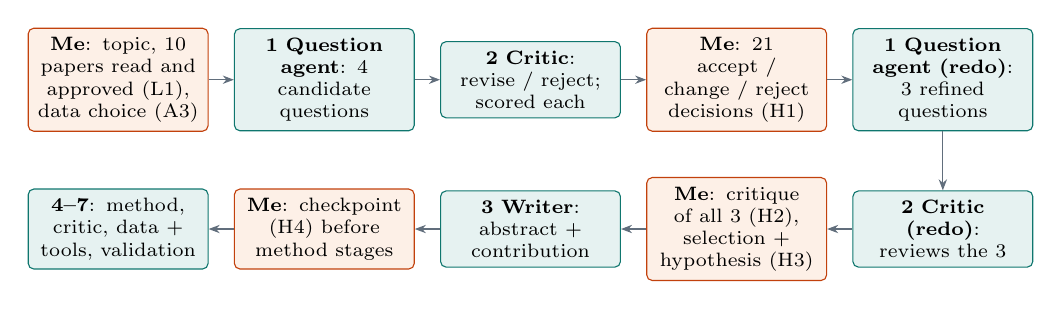
\begin{tikzpicture}[
  ag/.style={draw=teal,fill=tealtint,rounded corners=2pt,minimum height=0.85cm,text width=2.05cm,align=center,font=\scriptsize},
  me/.style={draw=amber,fill=ambertint,rounded corners=2pt,minimum height=0.85cm,text width=2.05cm,align=center,font=\scriptsize},
  ar/.style={-{Stealth[length=4pt]},color=muted},
  node distance=0.32cm]
\node[me] (a) {\textbf{Me}: topic, 10 papers read and approved (L1), data choice (A3)};
\node[ag,right=of a] (b) {\textbf{1 Question agent}: 4 candidate questions};
\node[ag,right=of b] (c) {\textbf{2 Critic}: revise / reject; scored each};
\node[me,right=of c] (d) {\textbf{Me}: 21 accept / change / reject decisions (H1)};
\node[ag,right=of d] (e) {\textbf{1 Question agent (redo)}: 3 refined questions};
\node[ag,below=0.75cm of e] (f) {\textbf{2 Critic (redo)}: reviews the 3};
\node[me,left=of f] (g) {\textbf{Me}: critique of all 3 (H2), selection + hypothesis (H3)};
\node[ag,left=of g] (h) {\textbf{3 Writer}: abstract + contribution};
\node[me,left=of h] (i) {\textbf{Me}: checkpoint (H4) before method stages};
\node[ag,left=of i] (j) {\textbf{4--7}: method, critic, data + tools, validation};
\foreach \x/\y in {a/b,b/c,c/d,d/e,e/f,f/g,g/h,h/i,i/j} \draw[ar] (\x) -- (\y);
\end{tikzpicture}

\vspace{8pt}
{\small \textcolor{amber}{\rule{8pt}{8pt}} human decision \qquad \textcolor{teal}{\rule{8pt}{8pt}} agent stage (fresh agent, given only a prompt packet) \qquad every output and packet archived}
\note{About 30 s. Each agent gets a self-contained packet built from my form; I decide at every orange box. Agreement between agents is not treated as validation.}
\end{frame}

% ------------------------------------------------------------------ 4
\begin{frame}[shrink=20]{Three refined questions and my critique}
\footnotesize
\begin{tabularx}{\textwidth}{@{}p{3.3cm}YYp{1.9cm}@{}}
\toprule
\textbf{Question} & \textbf{Scientific value (my critique)} & \textbf{Feasibility in 8 weeks (my critique)} & \textbf{Origin} \\
\midrule
\textbf{Q1.} Is a tool-using agent \emph{no worse} than a fixed pipeline with the same tools, better where the tools disagree, and does it abstain when data are missing?
 & Strong comparison. It is detection, not description, but tool outputs from classic CV methods act as extra features instead of the model interpreting from scratch.
 & Feasible at test level; a production system across many areas would take longer.
 & AI, edited by me \\
\addlinespace
\textbf{Q2.} Does 15\,m panchromatic add anything to Sentinel-1 SAR?
 & Good idea, but I would flip it: \alert{panchromatic supported by SAR}, since panchromatic is more common in commercial imagery.
 & Hard from scratch in 8 weeks; possible with an AI expert or by building on prior research.
 & AI, edited by me \\
\addlinespace
\textbf{Q3.} Does neighbouring-cell context help the agent place change in the right cell?
 & Reasonable, but too general: extra context could be almost anything, and it has no target problem.
 & Feasible.
 & AI \\
\bottomrule
\end{tabularx}
\note{About 40 s. These critiques are mine (H2). Q2's flip and Q3's rejection are my own changes.}
\end{frame}

% ------------------------------------------------------------------ 5
\begin{frame}[shrink=16]{Selected question: Q1}
\begin{block}{Research question}
In held-out SpaceNet 7 areas (2017--2020), does an LLM agent that answers questions about one 100\,m cell at a time, by calling fixed Sentinel-1 SAR and Landsat-8 panchromatic tools, detect new buildings \alert{at least as well as a fixed pipeline} with the same tools, do better where the tools disagree, and decline to answer when the data cannot support one?
\end{block}
\begin{columns}[T,onlytextwidth]
\column{0.48\textwidth}
\textbf{Why it is the strongest}
\begin{itemize}\small
  \item Both arms use the same tools, so any difference is the agent's reasoning.
  \item Feasible with existing labels; no model training.
  \item Q2 survives as a secondary, panchromatic-led analysis; Q3 dropped as too general.
\end{itemize}
\column{0.48\textwidth}
\textbf{Hypothesis}
\begin{itemize}\small
  \item Agent F1 for new-building cells is no worse than the pipeline's by more than a pre-set margin~$\delta$.
  \item Grounding in tools reduces hallucination: fewer fabricated answers than the same model without tools.
\end{itemize}
\end{columns}
\vspace{2pt}{\scriptsize \todo{make this slide match your final H3 wording}}
\note{About 35 s. Explain why the agent-vs-pipeline contrast isolates agency.}
\end{frame}

% ------------------------------------------------------------------ 6
\begin{frame}[shrink=14]{AI suggestions I accepted, changed or rejected}
\footnotesize
\begin{tabularx}{\textwidth}{@{}p{4.6cm}p{1.6cm}Y@{}}
\toprule
\textbf{AI suggestion} & \textbf{Decision} & \textbf{Why} \\
\midrule
Compare the agent with a direct vision-language model & \rej & Confounded and close to predetermined; a 100\,m cell is about 7\,$\times$\,7 panchromatic pixels. VLM arm dropped entirely. \\
Hand-label 300--500 cells; use NAIP for dates & \rej & SpaceNet 7 already has monthly building labels from separate imagery; saves about two weeks. \\
Archive-size factor (8 / 32 / all scenes) & \rej & True by construction: the VLM's input is capped. \\
Critic's revised question: agent vs fixed pipeline & \acc & The only contrast that isolates what the agent adds. \\
Panchromatic as an optional ablation & \chg & Required secondary analysis, and panchromatic-led (my Q2 critique). \\
Single area split into blocks & \chg & Whole areas held out (AOI-level split): less leakage, better external validity. \\
Neighbourhood-context question (Q3) & \rej & Too general; no target problem (my critique). \\
\bottomrule
\end{tabularx}
\vspace{3pt}{\scriptsize\color{muted} Full log: 21 decisions (form field H1); earlier outputs and every agent's input packet are archived.}
\note{About 35 s. This is the critical-review evidence: what I kept, changed and threw out, and why.}
\end{frame}

% ------------------------------------------------------------------ 7
\begin{frame}[shrink=14]{Literature and contribution}
\footnotesize
\begin{tabularx}{\textwidth}{@{}p{3.6cm}YY@{}}
\toprule
\textbf{Paper} & \textbf{What it established} & \textbf{What this work adds} \\
\midrule
Kao et al. (2026), ACL Findings & LLM agents on EO questions reach about 60\% at best; code generation often fails & Predefined, deterministic tools instead of free-form code \\
Feng et al. (2026), ICLR & Tool-using EO agent (Earth-Agent, 104 tools) & A SAR + panchromatic tool set and a same-tools baseline \\
Xuan et al. (2025), NeurIPS & MLLMs reach 34.1\% on long-term city change & Grounds answers in time-series statistics \\
Lee et al. (2026), IEEE JSTARS & SAR time-series change types; up-steps linked to construction & Uses the SAR change test inside an agent \\
Qu et al. (2026), Remote Sens. Environ. & Dense time-series change detection; AOI-level split; misalignment creates false change & Same split logic and misregistration checks \\
Zuo et al. (2026), IEEE JSTARS & Statistical calibration reduces hallucinated change claims & Measures abstention and fabricated answers \\
\bottomrule
\end{tabularx}
\vspace{4pt}
\textbf{Proposed contribution:} a controlled test of what the agentic layer adds over identical tools, on a dense SAR + panchromatic archive, scored against independent monthly labels. \alert{Proposed, not established.}
\note{About 30 s. All 10 references read and verified; full list in the supporting slides.}
\end{frame}

% ------------------------------------------------------------------ 8
\begin{frame}[shrink=18]{Data and method}
\begin{columns}[T,onlytextwidth]
\column{0.47\textwidth}
\textbf{Data (all public)}
\begin{itemize}\small
  \item \textbf{Panchromatic:} Landsat-8 band 8, 15\,m, monthly, already co-registered (MuRA-T, 60 SpaceNet 7 areas, 2017--2020)
  \item \textbf{SAR:} Sentinel-1 C-band GRD, one orbit track per area, co-registered by me
  \item \textbf{Reference:} SpaceNet 7 monthly building footprints, traced on separate PlanetScope imagery
  \item \textbf{Unit:} 100\,m cells in 10--20 areas; whole areas held out for testing
\end{itemize}
\column{0.49\textwidth}
\textbf{Steps}
\begin{enumerate}\small
  \item Build deterministic tools: SAR series and likelihood-ratio change test; normalised panchromatic series and change magnitude; data availability
  \item \textbf{Baseline:} fixed pipeline with the same tools, tuned on development areas
  \item \textbf{Agent:} same tools, answers \texttt{presence / onset month / abstain}
  \item Controls: same model without tools; panchromatic-only vs panchromatic + SAR
  \item Freeze, pre-register, run test areas once
\end{enumerate}
\textbf{AI-assisted coding:} Claude Code for tools, pipeline and agent harness; Python (rasterio, geopandas) and Earth Engine.
\end{columns}
\note{About 35 s. No model training. The baseline uses exactly the agent's tools.}
\end{frame}

% ------------------------------------------------------------------ 9
\begin{frame}[shrink=16]{Validation, spatial assumptions and risks}
\begin{columns}[T,onlytextwidth]
\column{0.48\textwidth}
\textbf{Validation checks}
\begin{itemize}\small
  \item Primary: agent F1 $\geq$ pipeline F1 $-\,\delta$, with an area-level cluster bootstrap CI
  \item Accuracy on cells where SAR and panchromatic disagree
  \item Abstention and fabricated-answer counts on unanswerable queries
  \item Robustness: 200\,m cells, one-pixel shift, look-direction tolerance
\end{itemize}
\textbf{Spatial assumptions}
\begin{itemize}\small
  \item Sub-pixel co-registration holds; cell size set in metres (grid may be Web Mercator)
  \item Labels mark when a building is visible, not when construction starts
\end{itemize}
\column{0.48\textwidth}
\begin{block}{What would weaken the claim}
\small
\begin{itemize}
  \item CI of (agent $-$ pipeline) extends below $-\delta$
  \item The no-tools model scores close to the agent (answers from memory)
  \item The agent almost never disagrees with the pipeline (then switch to the panchromatic question)
  \item Few test areas give wide CIs
\end{itemize}
\end{block}
\textbf{Key risks:} SAR layover moves signal between cells; Level-1 panchromatic radiometry adds false change; API budget.
\end{columns}
\note{About 35 s. Name one falsifier clearly.}
\end{frame}

% ------------------------------------------------------------------ 10
\begin{frame}[shrink=16]{Eight-week plan, journal and co-authors}
\begin{columns}[T,onlytextwidth]
\column{0.44\textwidth}
\footnotesize
\begin{tabular}{@{}lp{5.6cm}@{}}
\toprule
\textbf{Week} & \textbf{Work} \\
\midrule
1 & Download data, choose areas, draft pre-registration \\
2 & Grid and labels; build tools and pipeline \\
3 & Development runs; 20-cell pilot \\
4 & Freeze, pre-register, run test areas \\
5 & Analysis and robustness \\
6 & Draft paper \\
7 & Co-author review, revise \\
8 & Submit (buffer) \\
\bottomrule
\end{tabular}
\column{0.53\textwidth}
\textbf{Journal:} \emph{International Journal of Digital Earth} (Taylor \& Francis). JIF 5.4, 2025 JIF, Clarivate JCR (2026 release) \todo{verify in JCR}. Publishes AI-driven Earth observation and agentic GIS work; this paper takes that line to satellite time series.

\vspace{6pt}
\textbf{Possible co-authors} {\scriptsize(neither has agreed)}
\begin{itemize}\footnotesize
  \item \textbf{Dr.\ Edward Oughton}, GMU Geography \& Geoinformation Science: agentic GeoAI and spatial computing. Checks: workflow design, evaluation protocol, reproducibility.
  \item \textbf{Dr.\ Konrad Wessels}, GMU Geography \& Geoinformation Science: SAR and time-series remote sensing. Checks: SAR preprocessing, co-registration, physical plausibility of SAR change.
\end{itemize}
\end{columns}
\note{About 30 s. Plan detail is in the supporting slides.}
\end{frame}

% ------------------------------------------------------------------ 11
\begin{frame}{Sources and AI disclaimer}
\footnotesize
\textbf{Data:} MuRA-T (Purdue RVL; Deshmukh et al., 2023, arXiv:2302.12301, GPL v3); SpaceNet 7 (Van Etten et al., CVPR 2021, CC BY-SA 4.0); Copernicus Sentinel-1 (ESA); Landsat-8 (USGS). Full references: supporting slides.

\vspace{6pt}
\textbf{AI tools and what they did:} Claude Code (Anthropic, Claude Opus 5.5) built the orchestration script and prompt packets, ran each workflow role as a fresh agent (question, critic, writer, methodology, data + tools, validation), searched the literature and checked DOIs against Crossref, found the MuRA-T dataset, drafted the decision log (H1) and the data notes at my direction, and generated these slides.

\vspace{6pt}
\textbf{My own checks:} read and approved all 10 references; wrote my own critique of the three questions; selected the question and hypothesis; chose the journal and co-authors; reviewed the decision log \todo{confirm you reviewed and edited H1}; verified the journal metric \todo{after the JCR check}. Agreement between agents was not treated as validation.
\note{About 15 s.}
\end{frame}

% ------------------------------------------------------------------ 12
\begin{frame}[standout]
Questions?\\[6pt]
{\normalsize What does the agent add that the same tools do not?}
\end{frame}

\appendix
% ------------------------------------------------------------------ S1
\begin{frame}[shrink=10]{Supporting: full references (all read and verified)}
\scriptsize
\begin{itemize}
\item Feng, P., et al. (2026). Earth-Agent: Unlocking the full landscape of earth observation with agents. ICLR 2026. OpenReview: dkIXAbWuxO
\item Hou, Y., et al. (2026). SAR foundation models: A comprehensive review of data, models, and applications. Science China Information Sciences, 69(8), 180301. doi:10.1007/s11432-026-5040-3
\item Irvin, J. A., et al. (2025). TEOChat: A large vision-language assistant for temporal earth observation data. ICLR 2025. OpenReview: pZz0nOroGv
\item Kao, C.-H., et al. (2026). Towards LLM agents for earth observation. Findings of ACL 2026, 2597--2611. doi:10.18653/v1/2026.findings-acl.124
\item Lee, B., Lee, Y.-K., \& Kim, S.-W. (2026). Change type analysis for urban construction using time-series SAR data. IEEE JSTARS (early access). doi:10.1109/JSTARS.2026.3737141
\item Michel, J., \& Inglada, J. (2026). Temporal attention multi-resolution fusion of satellite image time-series, applied to Landsat-8/9 and Sentinel-2. Remote Sensing of Environment, 334, 115159. doi:10.1016/j.rse.2025.115159
\item Qu, Y., Li, J., \& Huang, X. (2026). AnyTime-CD: Self-supervised change detection in arbitrary-length dense time series of high-resolution remote sensing images. Remote Sensing of Environment, 334, 115239. doi:10.1016/j.rse.2026.115239
\item Soni, S., et al. (2025). EarthDial: Turning multi-sensory earth observations to interactive dialogues. CVPR 2025, 14303--14313. doi:10.1109/CVPR52734.2025.01334
\item Xuan, W., et al. (2025). DynamicVL: Benchmarking multimodal large language models for dynamic city understanding. NeurIPS 38 (Datasets and Benchmarks), 37321--37339. doi:10.52202/085713-1114
\item Zuo, L., et al. (2026). Hallucination-resistant change detection in multimodal large models for autonomous land management agents. IEEE JSTARS, 19, 6313--6327. doi:10.1109/JSTARS.2026.3656403
\end{itemize}
\textbf{Data sources:} Deshmukh, R., Roros, C. J., Kashyap, A., \& Kak, A. C. (2023). An aligned multi-temporal multi-resolution satellite image dataset for change detection research. arXiv:2302.12301 (preprint). \enskip Van Etten, A., et al. (2021). The Multi-Temporal Urban Development SpaceNet Dataset. CVPR 2021.
\end{frame}

% ------------------------------------------------------------------ S2
\begin{frame}[shrink=22]{Supporting: detailed eight-week plan}
\footnotesize
\begin{tabularx}{\textwidth}{@{}lYYY@{}}
\toprule
\textbf{Week} & \textbf{Tasks} & \textbf{Deliverable} & \textbf{Main risk} \\
\midrule
1 & Download MuRA-T, SpaceNet 7, Sentinel-1; inventory areas; feasibility check & Area list; draft pre-registration & Too few Sentinel-1 scenes in some areas \\
2 & 100\,m grid in metres; rasterise labels; build tools and fixed pipeline & Tool library; pipeline tuned on development areas & SAR co-registration error \\
3 & Development runs; 20-cell pilot (agreement, parse rate, tokens) & Prompt set; switch-rule decision & Agent rarely disagrees with pipeline \\
4 & Freeze; pre-register $\delta$, bands, thresholds; run test areas once & Raw results, run logs & API budget \\
5 & Scoring, bootstrap CIs, robustness (200\,m, shift, look direction) & Results tables and figures & Wide CIs with few areas \\
6 & Write the paper & Full draft & Scope creep \\
7 & Co-author review; revise & Revised draft & Reviewer-level gaps \\
8 & Submit to IJDE & Submission & Buffer only \\
\bottomrule
\end{tabularx}
\end{frame}

% ------------------------------------------------------------------ S3
\begin{frame}{Supporting: an agent output and my revision}
\small
\begin{columns}[T,onlytextwidth]
\column{0.48\textwidth}
\begin{block}{Agent (stage 1 redo), Q-B}
\footnotesize ``Does giving a tool-using LLM agent Landsat-8 panchromatic tools, in addition to Sentinel-1 tools, change how accurately it identifies 100\,m cells that gain new buildings?''
\end{block}
\begin{block}{Critic (stage 2), on the first draft}
\footnotesize Recommended keeping a direct vision-language model ``as descriptive context on a small subsample'', or dropping it.
\end{block}
\column{0.48\textwidth}
\begin{block}{My revision}
\footnotesize Flip the direction: \alert{panchromatic is the lead sensor, SAR supports it}, because panchromatic is more common in commercial imagery. Kept as a required secondary analysis inside Q1.
\end{block}
\begin{block}{My decision}
\footnotesize Dropped the vision-language model arm entirely: a 100\,m cell is about 7\,$\times$\,7 panchromatic pixels, and setting up the model would cost time the plan does not have.
\end{block}
\end{columns}
\vspace{4pt}{\scriptsize\color{muted} Outputs: \texttt{outputs/research\_questions.md}, \texttt{outputs/question\_review.md}; earlier versions and every prompt packet in \texttt{outputs/history/} and \texttt{outputs/packets\_used/}.}
\end{frame}

\end{document}
